\documentclass[table]{beamer}
\usepackage[utf8]{inputenc}
\usepackage[brazilian]{babel}
\usepackage{amsmath}
\usepackage{graphicx}
\usepackage{hyperref}
\usepackage{ragged2e}   
\usepackage{epstopdf}
\usepackage{multirow}
\usepackage{minted}
\usepackage{booktabs}

\setbeamertemplate{sidebar right}{}
\setbeamertemplate{footline}{%
\hfill\usebeamertemplate***{navigation symbols}
\hspace{1cm}\insertframenumber{}/\inserttotalframenumber}

\addtobeamertemplate{block begin}{}{\justifying}  %new code

\setbeamertemplate{footline}
{
  \leavevmode%
  \hbox{%
  \begin{beamercolorbox}[wd=.333333\paperwidth,ht=2.25ex,dp=1ex,center]{author in head/foot}%
    \usebeamerfont{author in head/foot}\insertsection
  \end{beamercolorbox}%
  \begin{beamercolorbox}[wd=.333333\paperwidth,ht=2.25ex,dp=1ex,center]{title in head/foot}%
    \usebeamerfont{title in head/foot}\insertsubsection
  \end{beamercolorbox}%
  \begin{beamercolorbox}[wd=.333333\paperwidth,ht=2.25ex,dp=1ex,right]{date in head/foot}%
    \usebeamerfont{date in head/foot}\insertshortdate{}\hspace*{2em}
    \insertframenumber{} / \inserttotalframenumber\hspace*{2ex} 
  \end{beamercolorbox}}%
  \vskip0pt%
}

\begin{document}

\begin{frame}
   \frametitle{Compiladores}
   \large
   \begin{center}
      Apresentação da Disciplina 
   \end{center}
   \scriptsize
   \begin{center}
      João Marcelo Uchôa de Alencar \\
      joao.marcelo@ufc.br \\
      UFC-Quixadá
   \end{center}
\end{frame}

\begin{frame}
   \tableofcontents
\end{frame}

\section{O Professor}
\begin{frame}
   \frametitle{O Professor}
   \begin{itemize}
      \item Prof. João Marcelo Uchôa de Alencar
      \item joao.marcelo@ufc.br
      \item \url{www.joao.marcelo.nom.br}
      \item Horário extra aula: quinta-feira, das 13:30 às 15:30 (enviar um e-mail antes).
   \end{itemize}
\end{frame}

\section{As Ferramentas}
\begin{frame}
   \frametitle{As Ferramentas}
   \begin{itemize}
      \item Slack:
      \begin{itemize}
         \item \url{https://compiladores20181.slack.com/};
	 \item ferramenta de colaboração muito usada por desenvolvedores de \textit{software};
	 \item comunicação \textbf{direta} com o professor;
	 \item os outros portais (SI3 e SIPPA) serão atualizados em uma frequência menor.
      \end{itemize}
      \item BitBucket:
      \begin{itemize}
         \item Controle de versão;
	 \item equivalente ao GitHub, porém permite projetos privados;
	 \item cada aluno já deve ir criando uma conta;
	 \item mais instruções a medida que os trabalhos de programação forem liberados.
      \end{itemize}
   \end{itemize}
   \begin{center}
   Ambas ferramentas são ótimas oportunidades para ir treinando o \textit{\textbf{Inglês}}!!!
   \end{center}
\end{frame}

\section{As Avaliações}
\begin{frame}
   \frametitle{As Avaliações}
   \begin{itemize}
      \item 4 notas:
      \begin{itemize}
         \item 3 avaliações escritas;
	 \item 1 nota dos trabalhos.
      \end{itemize}
      \item \textbf{nota final}: média das três maiores notas;
      \item proposta:
      \begin{itemize}
         \item se \textbf{nota final} $> 7.0$: aprovação garantida!
	 \item se \textbf{nota final} $< 7.0$ e \textbf{nota final} $> 5.0$: repito a média como nota da final, garantido aprovação.
	 \item se \textbf{nota final} $< 5.0$: reprovação.
      \end{itemize}
      \item concordam?
   \end{itemize}
\end{frame}

\begin{frame}
   \frametitle{Avaliações - Prova Escrita}
   \begin{itemize}
      \item Prova escrita tradicional, sem surpresas;
      \item no máximo discussões sobre algoritmos, sem questões envolvendo código;
      \item questões inspiradas nos livros de Compiladores disponíveis na biblioteca (mais sobre livros adiante).
   \end{itemize}
\end{frame}

\begin{frame}
   \frametitle{Avaliações - Trabalho}
   \begin{itemize}
      \item Trabalho incremental;
      \item um exercício de programação para cada etapa da construção de Compiladores;
      \item nenhuma ferramenta/linguagem é determinada, mas usar C e Lex/YACC facilita sua vida;
      \item a nota final será uma avaliação de todos os exercícios.
   \end{itemize}
\end{frame}

\section{O Conteúdo}
\begin{frame}
   \frametitle{Conteúdo Programático}   
   \hbox{\hspace{-1.35cm} 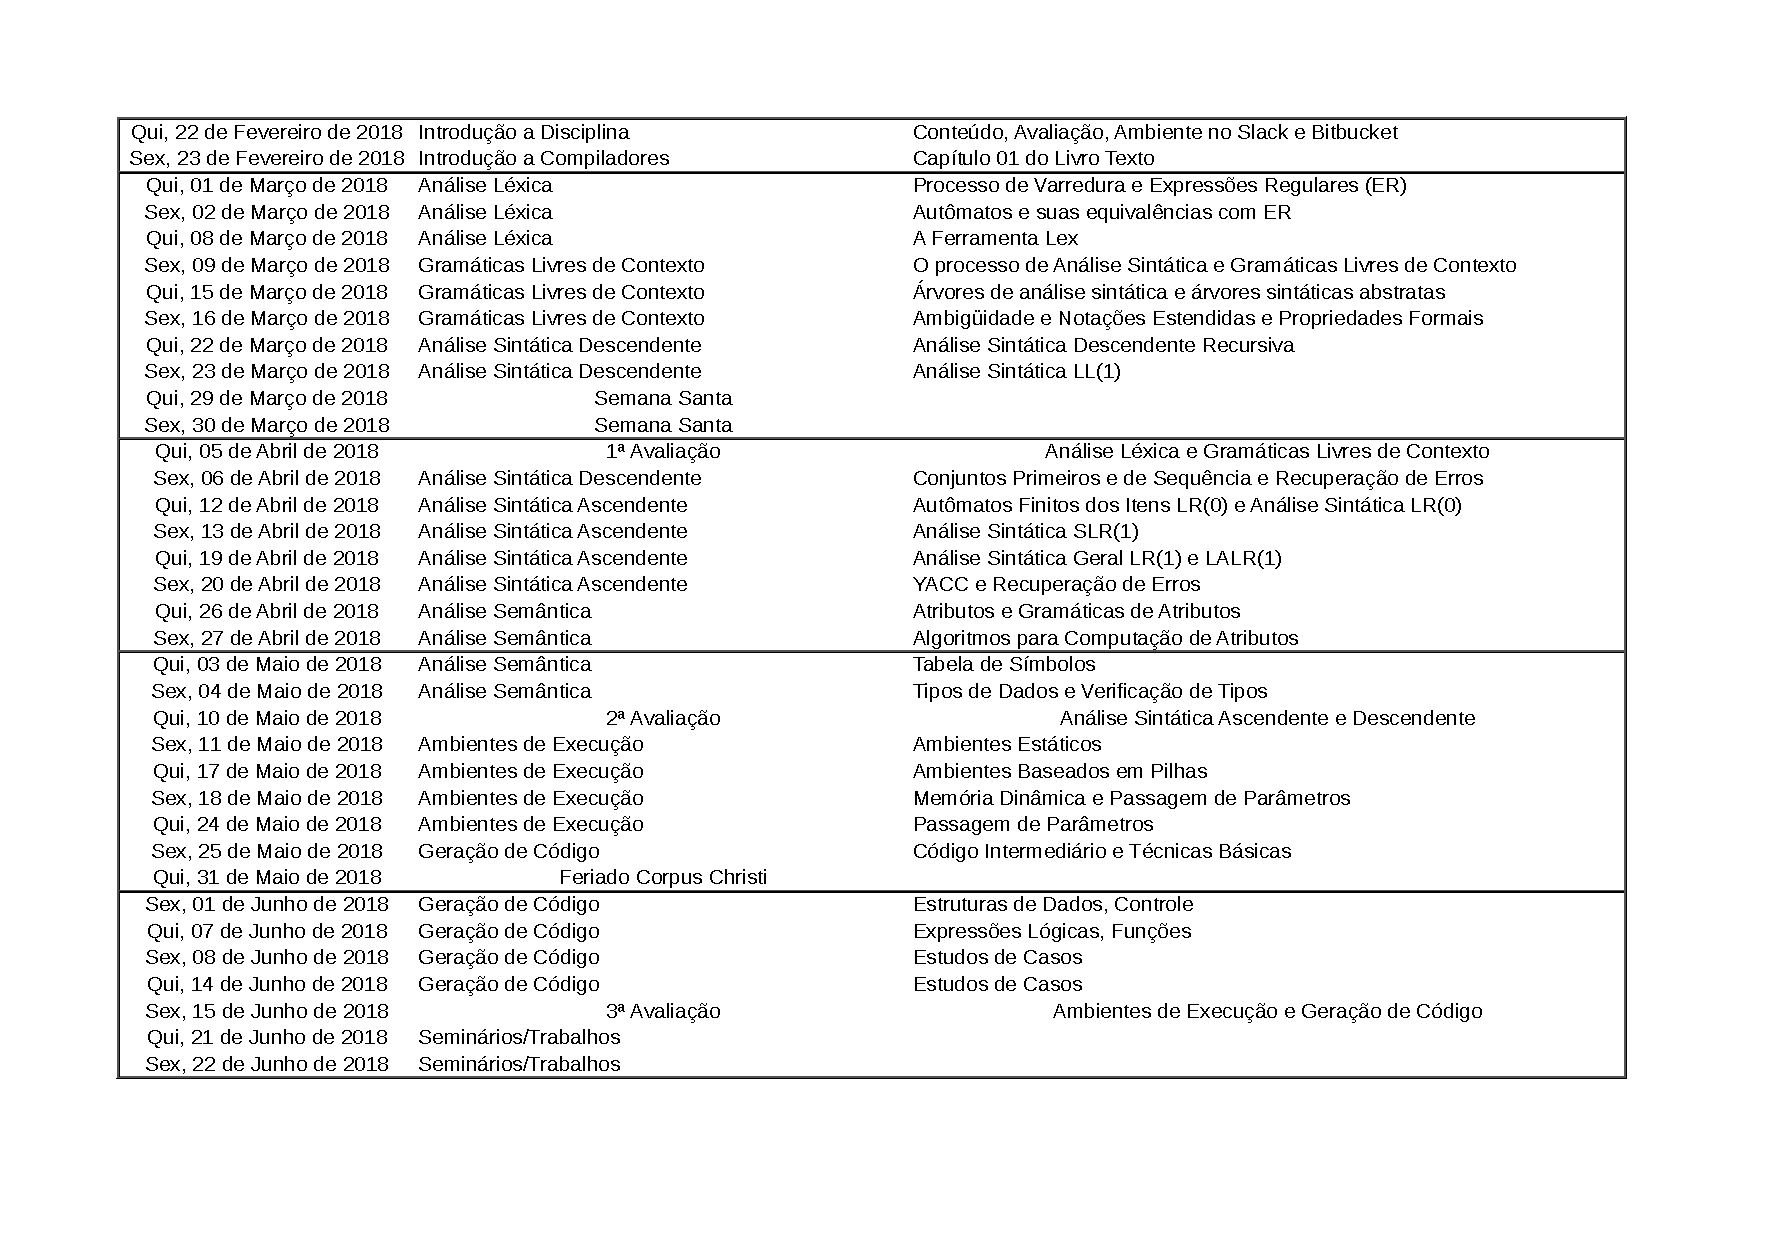
\includegraphics[scale=0.45]{figuras/programa.pdf}} 
\end{frame}

\begin{frame}
   \frametitle{Bibliografia - Base}
   \begin{columns}
      \begin{column}{0.5\textwidth}
         \begin{itemize}
	    \item Bibliografia Básica;
	    \item Compiladores Princípios e Práticas;
	    \item autor: Kenneth C. Louden;
	    \item 20 exemplares na biblioteca.
	 \end{itemize}
      \end{column}
      \begin{column}{0.5\textwidth}
      
\includegraphics[scale=1.0]{figuras/livro_base.jpg}
      \end{column}
   \end{columns}
\end{frame}

\begin{frame}
   \frametitle{Bibliografia - Auxiliar I}
   \begin{columns}
      \begin{column}{0.5\textwidth}
         \begin{itemize}
	    \item Bibliografia Clássica;
	    \item Compiladores Princípios, Técnicas e Ferramentas;
	    \item autor: Alfred V. Aho;
	    \item 32 exemplares na biblioteca.
	 \end{itemize}
      \end{column}
      \begin{column}{0.5\textwidth}
      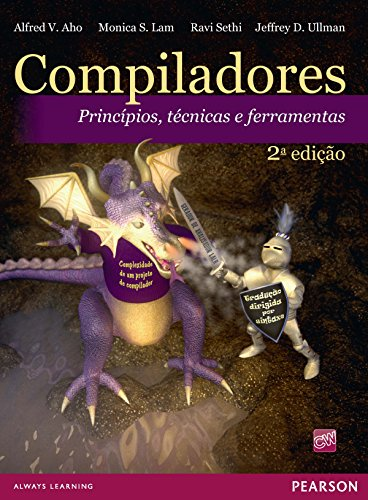
\includegraphics[scale=0.4]{figuras/livro_dragao.jpg}
      \end{column}
   \end{columns}
\end{frame}

\begin{frame}
   \frametitle{Bibliografia - Auxiliar II}
   \begin{columns}
      \begin{column}{0.5\textwidth}
         \begin{itemize}
	    \item Bibliografia Moderna;
	    \item Construindo Compiladores;
	    \item autores: Cooper e Torczon;
	    \item 1 exemplar na biblioteca.
	 \end{itemize}
      \end{column}
      \begin{column}{0.5\textwidth}
      
\includegraphics[scale=0.8]{figuras/livro_construindo.jpg}
      \end{column}
   \end{columns}
\end{frame}

\section{Dúvidas}
\begin{frame}
   \frametitle{Dúvidas?}
   Dúvidas? Sugestões?
\end{frame}
\end{document}
